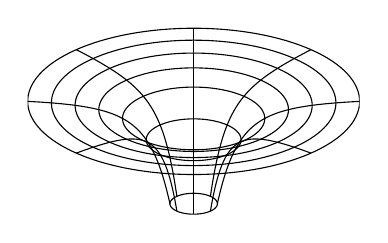
\begin{tikzpicture}

\begin{axis}[
view       = {0}{50},
axis lines = none,
% zmax       = 60,
height     = 5cm,
xtick      = \empty,
ytick      = \empty,
ztick      = \empty,
]
\foreach \i in {1, 2, ..., 7} {
	\addplot3+ [
		domain     = 0:360,
		samples    = 128,
		samples y  = 0,
		mark       = none,
		black,
		solid,
	] ( {\i*sin(x)},{\i*cos(x)},{-1/(\i^2 + 1)});
}
\foreach \i in {45, 90, ..., 360} {
	\addplot3+ [
		domain     = 1:7,
		samples    = 128,
		samples y  = 0,
		mark       = none,
		black,
		solid,
	] ({x*sin(\i)}, {x*cos(\i)}, {-1/(x^2 + 1)});
}
\end{axis}

\end{tikzpicture}